\documentclass[aspectratio=169,10pt]{beamer}

% Theme & Styling
\usetheme{Madrid}
\usecolortheme{beaver}
\setbeamertemplate{navigation symbols}{}
\setbeamertemplate{caption}[numbered]

% Packages
\usepackage{amsmath,amssymb}
\usepackage{booktabs}
\usepackage{graphicx}
\usepackage{tikz}
\usetikzlibrary{shapes.geometric, arrows, positioning, fit, backgrounds}
\usepackage{hyperref}
\usepackage{listings}
\usepackage{colortbl}

% Color definitions
\definecolor{primaryblue}{RGB}{26, 54, 93}
\definecolor{accentindigo}{RGB}{79, 70, 229}
\definecolor{softemerald}{RGB}{16, 185, 129}
\definecolor{warnamber}{RGB}{245, 158, 11}

\setbeamercolor{palette primary}{bg=primaryblue,fg=white}
\setbeamercolor{palette secondary}{bg=accentindigo,fg=white}
\setbeamercolor{titlelike}{parent=palette primary}
\setbeamercolor{structure}{fg=primaryblue}

% Title details
\title[Adaptive AI Companion]{Adaptive AI Companion for Academic Learning and Career Readiness}
\subtitle{B.Tech Final Year Capstone Project --- Phase 1 Review}
\author[Team TKM]{
  \textbf{Presented by:}\\
  Irene Rose Charles \quad Ameen Nujumudeen\\
  Vibha Edward Pereira \quad Al Ahaan
}
\institute[TKMIT]{
  Under the Guidance of: \textbf{Dr. Nijil Raj N}, Head of Department\\
  \vspace{0.2cm}
  Department of Computer Science and Engineering\\
  \textbf{TKM Institute of Technology, Kollam}
}
\date{October 2026}

\begin{document}

% ========================================================
% SLIDE 1: Title Slide
% ========================================================
\begin{frame}
  \titlepage
\end{frame}

% ========================================================
% SLIDE 2: Team Details & Roles
% ========================================================
\begin{frame}{Project Organization \& Team Details}
  \begin{table}[]
    \centering
    \small
    \begin{tabular}{lll}
      \toprule
      \textbf{Member Name} & \textbf{Register No.} & \textbf{Assigned Project Module} \\
      \midrule
      \textbf{Irene Rose Charles} & \textit{[Reg. No.]} & Team Lead, Knowledge Engine (RAG) \& PSM Hub \\
      \textbf{Dr. Nijil Raj N} & --- & Project Guide \& Head of Department, CSE \\
      \textbf{Ameen Nujumudeen} & \textit{[Reg. No.]} & Assessment Engine, Adaptive Testing \& Scoring \\
      \textbf{Vibha Edward Pereira} & \textit{[Reg. No.]} & Learning Analytics Engine, Mastery Modeling \\
      \textbf{Al Ahaan} & \textit{[Reg. No.]} & Career Readiness Engine, Resume \& Interview Prep \\
      \bottomrule
    \end{tabular}
  \end{table}
  \vspace{0.3cm}
  \begin{block}{Phase 1 Status}
    Architecture finalized, unified relational database models deployed, and the core Hub-and-Spoke Persistent Student Model integrated with initial engine implementations.
  \end{block}
\end{frame}

% ========================================================
% SLIDE 3: Abstract
% ========================================================
\begin{frame}{Abstract}
  \begin{itemize}
    \item \textbf{Core Innovation:} An integrated educational platform unifying academic learning, dynamic assessment, learning analytics, and career preparedness around a central \textbf{Persistent Student Model (PSM)}.
    \item \textbf{Four Collaborative AI Engines:}
      \begin{enumerate}
        \item \textbf{Knowledge Engine:} Verifiable, source-grounded question answering via Document Parsing and Retrieval-Augmented Generation (RAG).
        \item \textbf{Assessment Engine:} Adaptive diagnostic evaluations updating fine-grained concept mastery.
        \item \textbf{Learning Analytics Engine:} 0--100 continuous mastery quantification, weakness diagnosis, and transparent Explainable AI recommendations.
        \item \textbf{Career Development Engine:} Competency mapping against 6 industry roles, skill-gap analysis, automated resume auditing, and mock technical interview prep.
      \end{enumerate}
    \item \textbf{Decoupled Hub-and-Spoke Topology:} Engines communicate asynchronously through the PSM rather than direct peer-to-peer coupling, ensuring auditable state continuity and strict role-based data isolation.
  \end{itemize}
\end{frame}

% ========================================================
% SLIDE 4: Problem Statement
% ========================================================
\begin{frame}{Problem Statement}
  \begin{columns}[T]
    \begin{column}{0.48\textwidth}
      \begin{alertblock}{Fragmented Educational Silos}
        \begin{itemize}
          \item Learning Management Systems (LMS), online quiz portals, and career boards exist as isolated platforms.
          \item Student progress data is dispersed and ephemeral across semester boundaries.
        \end{itemize}
      \end{alertblock}
      \begin{alertblock}{Hallucination in Generic AI}
        \begin{itemize}
          \item General-purpose LLMs generate ungrounded responses with fabricated equations and untraceable sources.
        \end{itemize}
      \end{alertblock}
    \end{column}
    \begin{column}{0.48\textwidth}
      \begin{alertblock}{Lack of Topic-Level Mastery Insight}
        \begin{itemize}
          \item High-level letter grades obscure granular conceptual misconceptions (e.g., matrix chain rule vs. vanishing gradients).
        \end{itemize}
      \end{alertblock}
      \begin{alertblock}{Disconnected Career Preparation}
        \begin{itemize}
          \item Students lack visibility into how specific university coursework aligns with industry tech competencies and placement standards.
        \end{itemize}
      \end{alertblock}
    \end{column}
  \end{columns}
\end{frame}

% ========================================================
% SLIDE 5: Objectives and Scope
% ========================================================
\begin{frame}{Objectives and Scope}
  \begin{block}{Primary Objectives}
    \begin{enumerate}
      \item Implement a \textbf{Persistent Student Model} tracking knowledge state, weak concepts, and career trajectories.
      \item Build a \textbf{Source-Grounded Knowledge Engine} with strict citation verification and zero hallucinated references.
      \item Engineer an \textbf{Adaptive Assessment Engine} evaluating responses and updating topic mastery in real time.
      \item Develop a \textbf{Transparent Learning Analytics Engine} delivering Explainable AI recommendations.
      \item Implement a \textbf{Career Development Engine} with role matching, skill-gap analytics, and technical interview simulation.
      \item Enforce \textbf{Role-Based Access Control (RBAC)} across teacher classrooms and student enrollments.
    \end{enumerate}
  \end{block}
  \begin{exampleblock}{Project Scope}
    Targeted at undergraduate engineering curricula (demonstrated on B.Tech CSE AI \& ML coursework: CS401 Deep Learning and CS402 NLP \& RAG).
  \end{exampleblock}
\end{frame}

% ========================================================
% SLIDE 6: Four-Engine Architecture
% ========================================================
\begin{frame}{Proposed Solution: Hub-and-Spoke Architecture}
  \begin{center}
    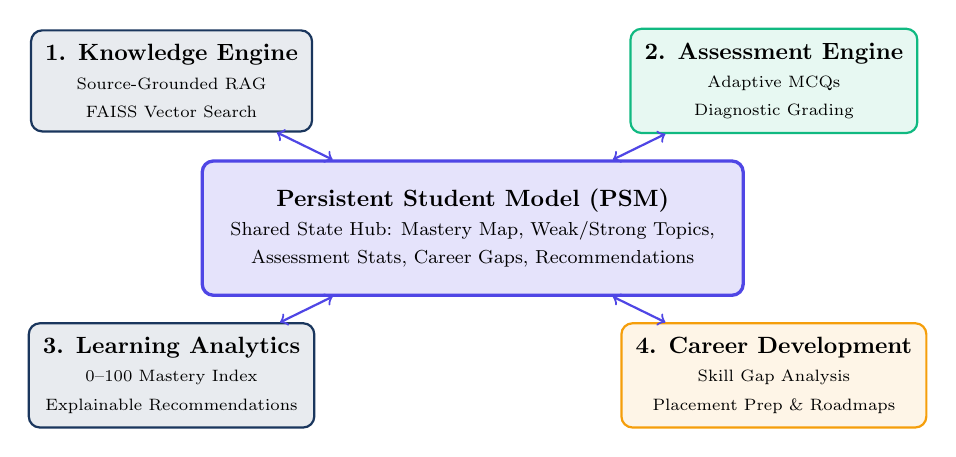
\begin{tikzpicture}[scale=0.85, every node/.style={transform shape}]
      % Center Hub
      \node (psm) [draw=accentindigo, fill=accentindigo!15, very thick, rounded corners, align=center, inner sep=12pt] at (0,0) {
        \textbf{Persistent Student Model (PSM)}\\
        \footnotesize Shared State Hub: Mastery Map, Weak/Strong Topics,\\
        \footnotesize Assessment Stats, Career Gaps, Recommendations
      };

      % Spokes
      \node (ke) [draw=primaryblue, fill=primaryblue!10, thick, rounded corners, align=center, inner sep=6pt] at (-4.5, 2.2) {
        \textbf{1. Knowledge Engine}\\
        \scriptsize Source-Grounded RAG\\
        \scriptsize FAISS Vector Search
      };
      \node (ae) [draw=softemerald, fill=softemerald!10, thick, rounded corners, align=center, inner sep=6pt] at (4.5, 2.2) {
        \textbf{2. Assessment Engine}\\
        \scriptsize Adaptive MCQs\\
        \scriptsize Diagnostic Grading
      };
      \node (la) [draw=primaryblue, fill=primaryblue!10, thick, rounded corners, align=center, inner sep=6pt] at (-4.5, -2.2) {
        \textbf{3. Learning Analytics}\\
        \scriptsize 0--100 Mastery Index\\
        \scriptsize Explainable Recommendations
      };
      \node (ce) [draw=warnamber, fill=warnamber!10, thick, rounded corners, align=center, inner sep=6pt] at (4.5, -2.2) {
        \textbf{4. Career Development}\\
        \scriptsize Skill Gap Analysis\\
        \scriptsize Placement Prep \& Roadmaps
      };

      % Connectors
      \draw[<->, thick, accentindigo] (ke) -- (psm);
      \draw[<->, thick, accentindigo] (ae) -- (psm);
      \draw[<->, thick, accentindigo] (la) -- (psm);
      \draw[<->, thick, accentindigo] (ce) -- (psm);
    \end{tikzpicture}
  \end{center}
  \footnotesize \textbf{Architectural Invariant:} Engines never communicate peer-to-peer. All reads and writes occur through backend PSM synchronization services, guaranteeing clean decoupling and multi-session continuity.
\end{frame}

% ========================================================
% SLIDE 7: Overall System Workflow
% ========================================================
\begin{frame}{Proposed Methodology: Overall Workflow}
  \begin{enumerate}
    \item \textbf{Classroom Setup:} Faculty creates class, generating a unique 7-character joining code (e.g., \texttt{DL4017A}), and uploads syllabus notes.
    \item \textbf{Document Ingestion:} Server extracts raw text (PyMuPDF/docx), divides it into semantic chunks with page metadata, computes embeddings, and indexes them in FAISS.
    \item \textbf{Student Enrollment:} Student enters code; system validates role permissions and establishes enrollment.
    \item \textbf{Source-Grounded Querying:} Knowledge Engine converts queries into dense vectors, retrieves matching chunks via cosine similarity, and formats responses with explicit page citations.
    \item \textbf{Assessment \& Mastery Update:} Student attempts adaptive diagnostic quizzes; Assessment Engine grades answers and writes evidence to the PSM.
    \item \textbf{Analytics \& Career Feedback:} Learning Analytics recomputes mastery ($0-100$ scale), updates weak/strong topic flags, and maps competencies to the Career Roadmap.
  \end{enumerate}
\end{frame}

% ========================================================
% SLIDE 8: Adaptive Learning Loop
% ========================================================
\begin{frame}{Proposed Methodology: Adaptive Learning Loop}
  \begin{columns}[T]
    \begin{column}{0.5\textwidth}
      \begin{block}{Continuous Learning Cycle}
        \begin{enumerate}
          \item \textbf{Baseline Assessment:} Diagnostic quiz establishes initial topic mastery.
          \item \textbf{Gap Identification:} Heuristics flag concepts falling below $55\%$ accuracy.
          \item \textbf{Targeted Recommendations:} PSM triggers focused revision tasks and adds them to the Study Planner.
          \item \textbf{Re-Assessment:} Higher difficulty testing verifies retention ($\ge 80\%$).
          \item \textbf{Competency Promotion:} Validated topics automatically promote to \textit{Inferred Skills} in the Career Profile.
        \end{enumerate}
      \end{block}
    \end{column}
    \begin{column}{0.48\textwidth}
      \begin{exampleblock}{Tripartite Evidence Model}
        The platform strictly separates:
        \begin{itemize}
          \item \textbf{Measured Performance:} Real, recorded test accuracy from completed quiz sessions.
          \item \textbf{Estimated Mastery:} Weighted exponential moving average ($0-100$).
          \item \textbf{Self-Reported Data:} Declared interests and skills, kept separate from inferred academic proof.
        \end{itemize}
      \end{exampleblock}
    \end{column}
  \end{columns}
\end{frame}

% ========================================================
% SLIDE 9: Literature Survey I — RAG
% ========================================================
\begin{frame}{Literature Survey I: Retrieval-Augmented Generation}
  \begin{block}{Lewis et al. (NeurIPS 2020) --- \textit{Retrieval-Augmented Generation for Knowledge-Intensive NLP Tasks}}
    \begin{itemize}
      \item \textbf{Core Premise:} Combines pre-trained parametric memory (generator LLM) with non-parametric memory (dense vector retrieval).
      \item \textbf{Mechanisms:} Uses Dense Passage Retrieval (DPR) to locate relevant evidence passages and conditions sequence generation on retrieved context.
      \item \textbf{Relevance to Knowledge Engine:} Serves as the foundational paradigm for querying syllabus PDFs without model hallucination.
      \item \textbf{Phase 1 Extension:} Incorporates strict citation verification where responses explicitly reference original document title, page number, and similarity score, with automated abstention when context is absent.
    \end{itemize}
  \end{block}
\end{frame}

% ========================================================
% SLIDE 10: Literature Survey II — Learning Analytics
% ========================================================
\begin{frame}{Literature Survey II: Learning Analytics \& Mastery Tracing}
  \begin{columns}[T]
    \begin{column}{0.48\textwidth}
      \begin{block}{Siemens \& Long (2011)}
        \textit{Penetrating the Fog: Analytics in Learning}
        \begin{itemize}
          \item Defined learning analytics as the measurement, collection, analysis, and reporting of learner data to optimize learning outcomes.
          \item Emphasized timely feedback loops over post-semester autopsies.
        \end{itemize}
      \end{block}
    \end{column}
    \begin{column}{0.48\textwidth}
      \begin{block}{Piech et al. (NeurIPS 2015)}
        \textit{Deep Knowledge Tracing}
        \begin{itemize}
          \item Modeled student knowledge progression using recurrent neural networks across sequential exercise interactions.
          \item Showed that granular topic-level modeling significantly outperforms aggregate exam scoring.
        \end{itemize}
      \end{block}
    \end{column}
  \end{columns}
  \vspace{0.2cm}
  \textbf{Our Project Synthesis:} Bridges document-grounded RAG, persistent topic-level mastery tracing, and workforce career competency gap analysis into a single unified architecture.
\end{frame}

% ========================================================
% SLIDE 11: Expected Outcomes
% ========================================================
\begin{frame}{Expected Project Outcomes}
  \begin{itemize}
    \item \textbf{Unified Academic Ecosystem:} Elimination of disjointed educational apps through a single, responsive dashboard.
    \item \textbf{Zero-Hallucination Question Answering:} Verification of source citations with strict abstention handling for missing curriculum data.
    \item \textbf{Dynamic Concept Mastery Modeling:} Accurate $0-100$ mastery index with transparent explainable AI rationale for student guidance.
    \item \textbf{Closed-Loop Study Assistance:} Integration of 4 personal note types (Text, Key-Point, Flashcards, Annotated Diagrams) with adaptive study schedules.
    \item \textbf{Placement Readiness & Roadmaps:} Structured 3-phase preparation paths, automated resume alignment scoring, and simulated technical interview practice.
    \item \textbf{Empirical Evaluation Benchmarks:} Retrieval precision/recall, assessment scoring reliability, and student usability metrics.
  \end{itemize}
\end{frame}

% ========================================================
% SLIDE 12: Tools and Technologies
% ========================================================
\begin{frame}{Tools, Technologies, and Implementation Stack}
  \begin{table}[]
    \centering
    \small
    \begin{tabular}{lll}
      \toprule
      \textbf{Component} & \textbf{Technology Stack} & \textbf{Implementation Role} \\
      \midrule
      \textbf{Frontend} & React 19, TypeScript, Tailwind CSS & Responsive SPA, Themes (Light/Dark/System) \\
      \textbf{Backend} & Python 3.11, FastAPI & Modular REST API, Pydantic validation \\
      \textbf{Database} & PostgreSQL, SQLAlchemy 2.0 & Relational tables, JSONB state persistence \\
      \textbf{Document Parser} & PyMuPDF, python-docx, python-pptx & PDF, Word, and Presentation text extraction \\
      \textbf{OCR} & Tesseract OCR & Text extraction from scanned academic diagrams \\
      \textbf{Embeddings} & Sentence Transformers (MiniLM/BGE) & Dense 384/768-dim vector representations \\
      \textbf{Vector Index} & FAISS (\texttt{IndexFlatL2} / \texttt{IndexIVFFlat}) & Fast nearest-neighbor similarity search \\
      \textbf{LLM Engine} & Google Gemini API (\texttt{gemini-2.5-flash}) & Source-grounded synthesis \& interview scoring \\
      \bottomrule
    \end{tabular}
  \end{table}
\end{frame}

% ========================================================
% SLIDE 13: Work Plan / Gantt Chart
% ========================================================
\begin{frame}{Project Schedule & Phase Milestones}
  \begin{table}[]
    \centering
    \small
    \begin{tabular}{lllll}
      \toprule
      \textbf{Project Milestones / Tasks} & \textbf{Phase 1} & \textbf{Phase 2} & \textbf{Phase 3} & \textbf{Phase 4} \\
      & \textit{(Aug--Oct)} & \textit{(Nov--Dec)} & \textit{(Jan--Feb)} & \textit{(Mar--Apr)} \\
      \midrule
      Requirements Gathering \& Literature Review & \cellcolor{softemerald!30}\textbf{Completed} & --- & --- & --- \\
      Hub-and-Spoke Architecture \& PSM Schema & \cellcolor{softemerald!30}\textbf{Completed} & Refinement & --- & --- \\
      Classroom Ingestion \& FAISS RAG Pipeline & \cellcolor{softemerald!30}\textbf{Completed} & Optimization & --- & --- \\
      Adaptive MCQ Testing \& 0-100 Mastery Index & \cellcolor{softemerald!30}\textbf{Completed} & Validation & --- & --- \\
      Career Readiness Pre-Assessment & Planned & \cellcolor{accentindigo!25}\textbf{In Progress} & --- & --- \\
      Empirical Evaluation \& Retrieval Benchmarks & --- & --- & \cellcolor{warnamber!25}\textbf{Planned} & --- \\
      Final Documentation, Report \& Defense & --- & --- & --- & \cellcolor{warnamber!25}\textbf{Planned} \\
      \bottomrule
    \end{tabular}
  \end{table}
\end{frame}

% ========================================================
% SLIDE 14: Mapping with Program Outcomes (POs)
% ========================================================
\begin{frame}{Mapping with Program Outcomes (POs)}
  \begin{table}[]
    \centering
    \small
    \begin{tabular}{llc}
      \toprule
      \textbf{PO} & \textbf{Contribution Description} & \textbf{Level} \\
      \midrule
      \textbf{PO1} (Engineering Knowledge) & Applied vector similarity, RAG, and Bayesian/weighted mastery math & \textbf{3} \\
      \textbf{PO2} (Problem Analysis) & Analyzed student learning friction and career competency deficits & \textbf{3} \\
      \textbf{PO3} (Design/Development) & Designed modular Hub-and-Spoke platform with 4 AI engines & \textbf{3} \\
      \textbf{PO5} (Modern Tool Usage) & Utilized React 19, FastAPI, FAISS, PyTorch, and Google Gemini API & \textbf{3} \\
      \textbf{PO8} (Ethics \& Privacy) & Isolated classroom records, RBAC permissions, and protected student notes & \textbf{2} \\
      \textbf{PO9} (Individual/Teamwork) & Coordinated parallel frontend, backend, and data modeling modules & \textbf{2} \\
      \textbf{PO10} (Communication) & Clear technical documentation, code documentation, and review presentation & \textbf{2} \\
      \bottomrule
    \end{tabular}
  \end{table}
  \footnotesize \textit{Scale: 1 = Low, 2 = Medium, 3 = High.}
\end{frame}

% ========================================================
% SLIDE 15: Mapping with Sustainable Development Goals (SDGs)
% ========================================================
\begin{frame}{Mapping with Sustainable Development Goals (SDGs)}
  \begin{columns}[T]
    \begin{column}{0.32\textwidth}
      \begin{block}{SDG 4: Quality Education}
        \small
        \begin{itemize}
          \item Enhances equitable access to high-quality academic support.
          \item Diagnoses misconceptions and personalizes practice at the student's individual pace.
        \end{itemize}
      \end{block}
    \end{column}
    \begin{column}{0.32\textwidth}
      \begin{block}{SDG 8: Decent Work \& Growth}
        \small
        \begin{itemize}
          \item Connects higher education directly with industry placement readiness.
          \item Identifies skill deficits for high-growth tech roles (ML, MLOps, Data Science).
        \end{itemize}
      \end{block}
    \end{column}
    \begin{column}{0.32\textwidth}
      \begin{block}{SDG 9: Industry \& Innovation}
        \small
        \begin{itemize}
          \item Pioneers an innovative educational software architecture combining semantic vector search and dynamic student modeling.
        \end{itemize}
      \end{block}
    \end{column}
  \end{columns}
\end{frame}

% ========================================================
% SLIDE 16: System Context & High-Level Architecture
% ========================================================
\begin{frame}{System Context \& Architectural Topology}
  \begin{center}
    \begin{tikzpicture}[scale=0.8, every node/.style={transform shape}]
      % Clients
      \node (teach) [draw, fill=amber!15, rounded corners, minimum width=2.4cm] at (-4, 2.8) {Faculty Browser};
      \node (stud) [draw, fill=blue!15, rounded corners, minimum width=2.4cm] at (-4, -2.8) {Student Browser};
      
      % Frontend
      \node (fe) [draw=primaryblue, fill=primaryblue!10, thick, rounded corners, minimum height=4cm, align=center] at (-1.5, 0) {
        \textbf{React 19 SPA}\\
        \scriptsize TypeScript, Vite\\
        \scriptsize Dashboard, Engines,\\
        \scriptsize Notes, Planner
      };

      % Backend Gateway
      \node (be) [draw=accentindigo, fill=accentindigo!10, thick, rounded corners, minimum height=4cm, align=center] at (1.8, 0) {
        \textbf{FastAPI Backend}\\
        \scriptsize JWT Auth \& RBAC\\
        \scriptsize REST Router Layer\\
        \scriptsize 4 Engine Services
      };

      % PSM Layer
      \node (psm) [draw=purple, fill=purple!15, very thick, rounded corners, align=center] at (5.5, 0) {
        \textbf{PSM Hub}\\
        \scriptsize Mastery Map\\
        \scriptsize Weak/Strong State
      };

      % Storage & AI
      \node (db) [draw, fill=gray!20, cylinder, shape border rotate=90, minimum height=1.5cm, align=center] at (9, 1.8) {
        \textbf{PostgreSQL}\\
        \scriptsize Relational \& JSONB
      };
      \node (faiss) [draw, fill=green!15, cylinder, shape border rotate=90, minimum height=1.5cm, align=center] at (9, -1.8) {
        \textbf{FAISS}\\
        \scriptsize Vector Index
      };
      \node (gemini) [draw=red, fill=red!10, rounded corners, align=center] at (1.8, -3.2) {
        \textbf{Google Gemini API}\\
        \scriptsize LLM Grounded Generation
      };

      % Connectors
      \draw[->, thick] (teach) -- (-2.4, 1.8);
      \draw[->, thick] (stud) -- (-2.4, -1.8);
      \draw[<->, very thick, primaryblue] (fe) -- (be) node[midway, above] {\scriptsize REST / JSON};
      \draw[<->, very thick, accentindigo] (be) -- (psm);
      \draw[<->, thick] (be) -- (db);
      \draw[<->, thick] (be) -- (faiss);
      \draw[<->, thick] (be) -- (gemini);
    \end{tikzpicture}
  \end{center}
\end{frame}

% ========================================================
% SLIDE 17: Role-Based User Workflows
% ========================================================
\begin{frame}{Role-Based User Workflows}
  \begin{columns}[T]
    \begin{column}{0.48\textwidth}
      \begin{block}{Faculty / Teacher Workflow}
        \begin{enumerate}
          \item \textbf{Authentication:} Sign in with faculty credentials.
          \item \textbf{Classroom Management:} Create course (e.g., CS401), generating unique 7-char join code.
          \item \textbf{Material Distribution:} Upload PDFs, lecture slides, and notes.
          \item \textbf{Enrollment Oversight:} Approve pending student requests or revoke access.
          \item \textbf{Class Analytics:} Inspect aggregate curriculum mastery and class-wide bottlenecks.
        \end{enumerate}
      \end{block}
    \end{column}
    \begin{column}{0.48\textwidth}
      \begin{block}{Student Workflow}
        \begin{enumerate}
          \item \textbf{Enrollment:} Join class using verified 7-character join code.
          \item \textbf{Knowledge Grounding:} Ask academic questions grounded in uploaded lecture files.
          \item \textbf{Assessment Practice:} Take topic-targeted adaptive quizzes; review explanations.
          \item \textbf{Personal Workspace:} Create notes (Text, Key-Point, Flashcard, Diagram) and study tasks.
          \item \textbf{Career Exploration:} Review skill gaps and practice simulated technical interviews.
        \end{enumerate}
      \end{block}
    \end{column}
  \end{columns}
\end{frame}

% ========================================================
% SLIDE 18: Knowledge Engine: Document Ingestion Pipeline
% ========================================================
\begin{frame}{Knowledge Engine: Document Ingestion Pipeline}
  \begin{center}
    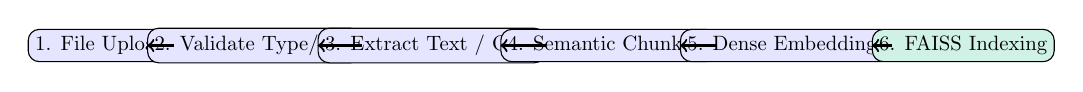
\begin{tikzpicture}[node distance=1.2cm, auto, scale=0.75, every node/.style={transform shape}]
      \node (up) [draw, rounded corners, fill=blue!10] {1. File Upload};
      \node (val) [draw, rounded corners, fill=blue!10, right of=up, node distance=2.6cm] {2. Validate Type/Size};
      \node (ext) [draw, rounded corners, fill=blue!10, right of=val, node distance=3cm] {3. Extract Text / OCR};
      \node (chk) [draw, rounded corners, fill=blue!10, right of=ext, node distance=3cm] {4. Semantic Chunking};
      \node (emb) [draw, rounded corners, fill=blue!10, right of=chk, node distance=3cm] {5. Dense Embeddings};
      \node (idx) [draw, rounded corners, fill=softemerald!20, right of=emb, node distance=3cm] {6. FAISS Indexing};

      \path[->, thick] (up) edge (val);
      \path[->, thick] (val) edge (ext);
      \path[->, thick] (ext) edge (chk);
      \path[->, thick] (chk) edge (emb);
      \path[->, thick] (emb) edge (idx);
    \end{tikzpicture}
  \end{center}
  \begin{itemize}
    \item \textbf{Supported Formats:} PDF (via PyMuPDF), DOCX (via python-docx), PPTX (via python-pptx), and Scanned Images (Tesseract OCR).
    \item \textbf{Metadata Preservation:} Each chunk stores original document ID, course ID, page/slide number, and unique FAISS vector identifier.
    \item \textbf{Semantic Chunking:} Employs 500-token chunks with 50-token overlapping boundaries to maintain contextual coherence across sentence splits.
  \end{itemize}
\end{frame}

% ========================================================
% SLIDE 19: Knowledge Engine: RAG Retrieval & Grounding
% ========================================================
\begin{frame}{Knowledge Engine: RAG Retrieval \& Grounding}
  \begin{center}
    \footnotesize
    \texttt{Query $\to$ Auth Filter $\to$ Embeddings $\to$ FAISS Top-K $\to$ Context Construction $\to$ LLM $\to$ Citations}
  \end{center}
  \begin{columns}[T]
    \begin{column}{0.48\textwidth}
      \begin{block}{Security \& Retrieval Constraints}
        \begin{itemize}
          \item \textbf{Enrollment Scoping:} Vector search is strictly partitioned to chunks belonging to student's active classes (prevents cross-course leakage).
          \item \textbf{Vector Distance:} Cosine similarity threshold ($s \ge 0.20$) filters out non-relevant context.
        \end{itemize}
      \end{block}
    \end{column}
    \begin{column}{0.48\textwidth}
      \begin{block}{Verifiable Source Citations}
        \begin{itemize}
          \item Every generated answer includes explicit citations: \texttt{[Source: Lecture\_01.pdf, Page 4]}.
          \item \textbf{Strict Anti-Hallucination:} If no chunks exceed threshold, returns: \textit{``The requested information was not found in your available course materials.''}
        \end{itemize}
      \end{block}
    \end{column}
  \end{columns}
\end{frame}

% ========================================================
% SLIDE 20: Assessment Engine & Mastery Estimation
% ========================================================
\begin{frame}{Assessment Engine \& Mastery Estimation Formula}
  \begin{block}{Dynamic MCQ Generation & Diagnostic Testing}
    Synthesizes questions parameterized by \textbf{Topic}, \textbf{Difficulty} (Beginner, Intermediate, Advanced), and \textbf{Count} (3, 5, 10), providing immediate pedagogical explanations upon submission.
  \end{block}
  \begin{exampleblock}{Normalized Mastery Estimation Model}
    Topic mastery $M_t \in [0, 100]$ is computed dynamically using a weighted exponential moving average:
    \begin{equation*}
      M_t = \alpha \cdot M_{t-1} + (1 - \alpha) \cdot \left[ w_1 A_t + w_2 D_t + w_3 C_t + w_4 P_t \right]
    \end{equation*}
    \small
    \begin{itemize}
      \item $M_{t-1}$: Historical baseline mastery estimate (retained in PSM).
      \item $A_t$: Raw accuracy percentage on current assessment.
      \item $D_t$: Difficulty modifier ($1.0$ for Beginner, $1.15$ for Intermediate, $1.30$ for Advanced).
      \item $C_t$: Streak consistency factor across consecutive test attempts.
      \item $P_t$: Progress velocity (derivative of performance over recent assessment window).
      \item Phase 1 Operational Weights: $\alpha = 0.40, (1-\alpha) = 0.60$ for immediate responsive feedback.
    \end{itemize}
  \end{exampleblock}
\end{frame}

% ========================================================
% SLIDE 21: Career-Readiness Pre-Assessment
% ========================================================
\begin{frame}{Career-Readiness Pre-Assessment}
  \begin{columns}[T]
    \begin{column}{0.48\textwidth}
      \begin{block}{Evaluation Dimensions}
        \begin{enumerate}
          \item \textbf{Academic Foundation:} Prerequisite mathematical and algorithmic comprehension.
          \item \textbf{General Aptitude:} Quantitative analysis, logical reasoning, and pattern recognition.
          \item \textbf{Role Knowledge:} Core tools (PyTorch, Docker, FAISS, LangChain, Transformers).
          \item \textbf{Self-Reported Experience:} Declared skills, github projects, and career preferences.
        \end{enumerate}
      \end{block}
    \end{column}
    \begin{column}{0.48\textwidth}
      \begin{block}{Readiness Deliverables}
        \begin{itemize}
          \item \textbf{Target Role Matching:} Comparison against 6 standardized profiles (ML, AI, NLP, CV, Data Science, MLOps).
          \item \textbf{Role Match Percentage:} Quantitative alignment rating ($0-100\%$).
          \item \textbf{Phased Action Plan:} 3-month structured roadmap targeting high-priority skill gaps.
          \item \textbf{Technical Interview Module:} Interactive text-based technical coding/system questions with automated rubric feedback.
        \end{itemize}
      \end{block}
    \end{column}
  \end{columns}
\end{frame}

% ========================================================
% SLIDE 22: Persistent Student Model (PSM) Schema
% ========================================================
\begin{frame}{Persistent Student Model (PSM) Schema}
  \begin{table}[]
    \centering
    \small
    \begin{tabular}{llp{7.5cm}}
      \toprule
      \textbf{Information Group} & \textbf{Data Structure} & \textbf{Attributes \& Functional Purpose} \\
      \midrule
      \textbf{Identity \& Profile} & Relational & Student ID, program (B.Tech CSE AI), semester, active enrollments \\
      \textbf{Knowledge State} & JSONB Map & Topic keys, $0-100$ mastery score, total attempts, status \\
      \textbf{Diagnostic Gaps} & JSONB Array & Identified weak topics ($<55\%$), failure reasons, recommended actions \\
      \textbf{Mastered Strengths} & JSONB Array & Topics with consistent high scores ($\ge 80\%$) across multiple quizzes \\
      \textbf{Assessment History} & JSONB Array & Timestamped scores, accuracy, time spent, question breakdown \\
      \textbf{Career Profile} & JSONB Object & Target role, declared skills, inferred academic skills, missing gaps \\
      \textbf{Next Best Action} & JSONB Object & Urgent/High priority task with Explainable AI evidence \\
      \textbf{Audit Trail} & JSONB Array & Timestamped synchronization log across all 4 AI engines \\
      \bottomrule
    \end{tabular}
  \end{table}
\end{frame}

% ========================================================
% SLIDE 23: Data Flow & Engine Integration
% ========================================================
\begin{frame}{Data Flow \& Engine Integration}
  \begin{center}
    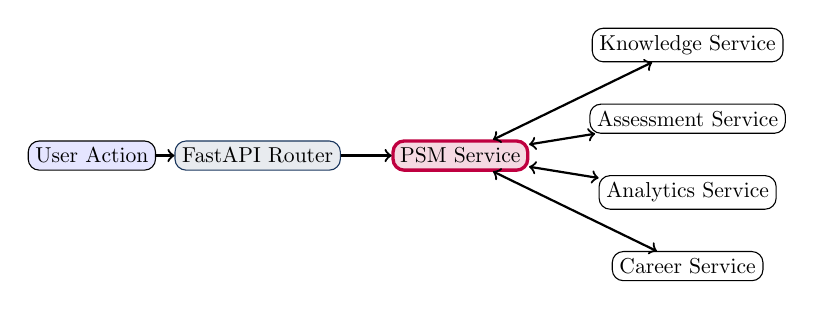
\begin{tikzpicture}[scale=0.78, every node/.style={transform shape}]
      \node (client) [draw, fill=blue!10, rounded corners] at (-4.5, 0) {User Action};
      \node (api) [draw=primaryblue, fill=primaryblue!10, rounded corners] at (-1.8, 0) {FastAPI Router};
      \node (psm) [draw=purple, fill=purple!15, very thick, rounded corners] at (1.5, 0) {PSM Service};
      
      \node (ke) [draw, rounded corners] at (5.2, 1.8) {Knowledge Service};
      \node (ae) [draw, rounded corners] at (5.2, 0.6) {Assessment Service};
      \node (la) [draw, rounded corners] at (5.2, -0.6) {Analytics Service};
      \node (ce) [draw, rounded corners] at (5.2, -1.8) {Career Service};

      \draw[->, thick] (client) -- (api);
      \draw[->, thick] (api) -- (psm);
      \draw[<->, thick] (psm) -- (ke);
      \draw[<->, thick] (psm) -- (ae);
      \draw[<->, thick] (psm) -- (la);
      \draw[<->, thick] (psm) -- (ce);
    \end{tikzpicture}
  \end{center}
  \begin{itemize}
    \item \textbf{Atomic Updates:} Assessment submissions execute atomic transactions updating test attempts, recalculating mastery, and logging audit events in a single pass.
    \item \textbf{Explainable Trail:} Every recommendation links back to verifiable database entries (e.g., \textit{``Accuracy dropped to 40\% on Backpropagation quiz on Oct 10''}).
  \end{itemize}
\end{frame}

% ========================================================
% SLIDE 24: Backend Architecture Layers
% ========================================================
\begin{frame}{Backend Architecture Layers}
  \begin{columns}[T]
    \begin{column}{0.48\textwidth}
      \begin{block}{Layered Architecture}
        \begin{enumerate}
          \item \textbf{API Routing Layer:} Handles HTTP validation via Pydantic schemas (\texttt{auth}, \texttt{classrooms}, \texttt{knowledge}, \texttt{assessment}, \texttt{analytics}, \texttt{career}, \texttt{notes}).
          \item \textbf{Authentication Layer:} Issues JWT Bearer tokens and verifies role-based permissions (Teacher vs. Student).
          \item \textbf{Service Layer:} Decoupled business logic (\texttt{PSMBackendService}, \texttt{RAGBackendService}).
          \item \textbf{Data Access Layer:} SQLAlchemy 2.0 ORM with PostgreSQL database engine.
        \end{enumerate}
      \end{block}
    \end{column}
    \begin{column}{0.48\textwidth}
      \begin{block}{Implementation Structure}
        \footnotesize
        \texttt{backend/app/}\\
        \texttt{\phantom{X}├── main.py \quad (FastAPI App, CORS)}\\
        \texttt{\phantom{X}├── config.py \quad (Environment)}\\
        \texttt{\phantom{X}├── database.py \quad (SQLAlchemy Engine)}\\
        \texttt{\phantom{X}├── models.py \quad (PostgreSQL Tables)}\\
        \texttt{\phantom{X}├── schemas.py \quad (Pydantic Models)}\\
        \texttt{\phantom{X}├── routers/ \quad (Modular Endpoints)}\\
        \texttt{\phantom{X}└── services/ \quad (PSM, RAG, Analytics)}
      \end{block}
    \end{column}
  \end{columns}
\end{frame}

% ========================================================
% SLIDE 25: Database Design and Core Entities
% ========================================================
\begin{frame}{Database Design & Core Relational Entities}
  \begin{columns}[T]
    \begin{column}{0.48\textwidth}
      \small
      \textbf{Core Entities Implemented:}
      \begin{itemize}
        \item \texttt{User}: \textit{id, name, email, role, password\_hash, degree\_program, semester}
        \item \texttt{Classroom}: \textit{id, name, subject, join\_code (7-char), teacher\_id}
        \item \texttt{ClassEnrollment}: \textit{id, class\_id, student\_id, status (active/pending/removed)}
        \item \texttt{LearningMaterial}: \textit{id, class\_id, title, file\_type, chunk\_count}
        \item \texttt{MaterialChunk}: \textit{id, material\_id, page\_num, content, faiss\_vector\_id}
      \end{itemize}
    \end{column}
    \begin{column}{0.48\textwidth}
      \small
      \textbf{Assessment \& Workspace Entities:}
      \begin{itemize}
        \item \texttt{PersistentStudentModel}: \textit{id, student\_id, knowledge\_mastery\_map, weak\_topics, career\_profile, next\_action}
        \item \texttt{Assessment}: \textit{id, student\_id, topic, difficulty, score, accuracy}
        \item \texttt{AssessmentResponse}: \textit{id, assess\_id, selected\_option, is\_correct, explanation}
        \item \texttt{PersonalNote}: \textit{id, student\_id, note\_type, title, content\_json, tags}
        \item \texttt{StudyTask}: \textit{id, student\_id, title, scheduled\_date, completed}
      \end{itemize}
    \end{column}
  \end{columns}
\end{frame}

% ========================================================
% SLIDE 26: Security, Privacy, and Authorization
% ========================================================
\begin{frame}{Security, Privacy, and Authorization}
  \begin{itemize}
    \item \textbf{Strict Class Boundary Isolation:} Students cannot query, view, or retrieve FAISS vector chunks from classrooms where their enrollment is not actively approved.
    \item \textbf{Enrollment Revocation Enforcement:} Revoking a student's enrollment immediately invalidates their access tokens and purges them from course material queries.
    \item \textbf{Privacy-Preserving Faculty View:} Teachers can monitor class-wide topic averages and difficulty trends, but have zero access to students' private personal study notes or career roadmaps.
    \item \textbf{Server-Side Credential Isolation:} LLM API keys and database credentials reside strictly on the server backend; zero sensitive keys exposed to browser clients.
    \item \textbf{Safe Input Validation:} Enforces file format and size limits, input sanitization against prompt injection, and host header validation (\texttt{allowedHosts: true}).
  \end{itemize}
\end{frame}

% ========================================================
% SLIDE 27: References I
% ========================================================
\begin{frame}{References}
  \footnotesize
  \begin{enumerate}
    \item Lewis, P., Perez, E., Piktus, A., Petroni, F., Karpukhin, V., Goyal, N., K\"uttler, H., Lewis, M., Yih, W.-t., Rockt\"aschel, T., Riedel, S., \& Kiela, D. (2020). Retrieval-augmented generation for knowledge-intensive NLP tasks. \textit{Advances in Neural Information Processing Systems (NeurIPS 2020)}, 33, 9459--9474.
    \item Siemens, G., \& Long, P. (2011). Penetrating the fog: Analytics in learning and education. \textit{EDUCAUSE Review}, 46(5), 30--40.
    \item Piech, C., Bassen, J., Huang, J., Ganguli, S., Sahami, M., Guibas, L. J., \& Sohl-Dickstein, J. (2015). Deep knowledge tracing. \textit{Advances in Neural Information Processing Systems (NeurIPS 2015)}, 28.
    \item Devlin, J., Chang, M.-W., Lee, K., \& Toutanova, K. (2019). BERT: Pre-training of deep bidirectional transformers for language understanding. \textit{Proceedings of NAACL-HLT 2019}, 4171--4186.
  \end{enumerate}
\end{frame}

% ========================================================
% SLIDE 28: References II
% ========================================================
\begin{frame}{References}
  \footnotesize
  \begin{enumerate}
    \setcounter{enumi}{4}
    \item Vaswani, A., Shazeer, N., Parmar, N., Uszkoreit, J., Jones, L., Gomez, A. N., Kaiser, \L., \& Polosukhin, I. (2017). Attention is all you need. \textit{Advances in Neural Information Processing Systems (NeurIPS 2017)}, 30.
    \item Johnson, J., Douze, M., \& J\'egou, H. (2019). Billion-scale similarity search with GPUs. \textit{IEEE Transactions on Big Data}, 7(3), 535--547.
    \item OWASP Foundation. (2024). \textit{OWASP Top 10 for Large Language Model Applications}. Open Web Application Security Project.
    \item United Nations. (2015). \textit{Transforming our world: The 2030 Agenda for Sustainable Development}. United Nations General Assembly Resolution A/RES/70/1.
  \end{enumerate}
\end{frame}

% ========================================================
% SLIDE 29: Current Status & Phase 2 Next Steps
% ========================================================
\begin{frame}{Current Status & Phase 2 Road Ahead}
  \begin{columns}[T]
    \begin{column}{0.48\textwidth}
      \begin{block}{Phase 1 Achievements Completed}
        \begin{itemize}
          \item Full Hub-and-Spoke architecture designed and implemented in code.
          \item PostgreSQL database schema and SQLAlchemy models deployed.
          \item 7-character classroom enrollment protocol operational.
          \item All 4 AI engines wired to the Persistent Student Model.
          \item RAG pipeline grounded on B.Tech AI course syllabus notes.
          \item Light/Dark/System theme system and live PSM inspector.
        \end{itemize}
      \end{block}
    \end{column}
    \begin{column}{0.48\textwidth}
      \begin{block}{Phase 2 Planned Objectives}
        \begin{itemize}
          \item Integrate multidimensional Career-Readiness Pre-Assessment questionnaire.
          \item Fine-tune FAISS vector index parameters (\texttt{nprobe}, \texttt{IndexIVFFlat}) on larger textbook corpora.
          \item Conduct student cohort usability evaluation and measure citation precision.
          \item Prepare mid-phase technical paper and experimental benchmark report.
        \end{itemize}
      \end{block}
    \end{column}
  \end{columns}
  \vspace{0.3cm}
  \begin{center}
    \textbf{Thank you! Questions and feedback are welcome.}
  \end{center}
\end{frame}

\end{document}
